\chapter{Literature reviews}

\section{Problem statement}
\label{sec:problem-statement}

The problem is as follows: consider a solenoid of length $L$, radius $R$, made from copper wire with resistivity $\Omega$, wound into $K$ layers, each consisting of $N$ loops. A free-falling Amperian magnet of length $\mathcal{l}$, mass $M$, and magnetic dipole moment $\mu$ is dropped from a height $z_0$ through the center of the solenoid. From the induced electromotive force $\emf$, is possible to determine Earth's gravitational constant by analyzing the voltage difference alone?

To solve this problem, the first step is to calculate the magnetic flux, $\mflux$, through the solenoid. Once the flux is known, the induced current and electromotive force, which are all functions of the magnet's position and velocity, can be determined. With the induced current, Lenz's law determines the force acting on the magnet. Finally, Newton's law is applied to combine this force with Earth's gravitational force into a differential equation that describes the magnet's position and velocity.

Since the magnet's velocity is a function of gravity, and the voltage is a function of velocity, Earth's gravity can be directly determined by measuring the voltage. However, the data is complex to process, so we focus on the minima of the voltage, which can be directly measured using an oscilloscope. By fitting this minimum voltage to the expected function, we can accurately calculate the gravitational force.

However, we will see in \cref{sec:perfect-magnetic-dipole} that the force contribution from Lenz's law makes the problem in its full form is not analytically solvable. Therefore, some simplifications must be made for an analytical solution to be viable.

\section{Related works}
\label{sec:related-works}

From my current knowledge, three studies have addressed the measurement of Earth's gravitational acceleration via electromagnetic induction. \emph{Ahmad Khan, Amar} \lcite{khan-no-date} has conducted a similar experiment but relied on numerical solutions of the entire voltage function without the effect from Lenz's law. \emph{Riad, Ihaf F.} \lcite{riad-2023} had performed a comparable experiment but with multiple solenoids to capture the difference in time between each coil's induction, with a long tube guiding the magnet's descent. Lastly, \emph{Jing, Liu} \lcite{jing-2019} succeeded to measure Earth's gravitational acceleration by using two solenoids that functions like a traditional photogate. However, none of these studies have included the magnet's retardation effect from Lenz's law yet.

\section{Simplification of problem}

The problem is simplified as follows: the finite-length solenoid is replaced with a solenoid with zero length, wounded around $N$ times, and the Amperian magnet is replaced by a perfect magnetic dipole with magnetic moment coefficient $\mu$. Funnily, this problem is still unsolvable analytically. So, we would have to resort to either neglection of terms or numerical methods. In this study, we've chosen not to neglect the Lenz's law, but to compare the results observed with the simulated theoretical voltage difference in order to find Earth's gravitational acceleration.

\section{Induction from a perfect magnetic dipole}
\label{sec:perfect-magnetic-dipole}

First, let's evaluate the magnetic flux on a loop. Let there be a magnet with a magnetic moment $\vv{m}$ pointing downwards ($\vv{m} = m\zhat$) situated at $z(t = 0) = h$. The magnetic flux is given by
\begin{equation}
	\mflux = \sint \vv{B}(\brc) \vdot \odif{\vv{A}}.
\end{equation}
The surface area vector element $\odif{\vv{A}}$ is defined as $\nhat\odif{A}$, where $\nhat$ is a vector normal to the surface of integration. In a cylindrical coordinate $(\rho, \theta, z)$ with the area integration element $\rho\odif{\rho}\odif{\theta}$,
\begin{equation}
	\odif{\vv{A}} = \nhat\rho\odif{\rho}\odif{\theta};
\end{equation}
hence,
\begin{equation}
	\mflux = \sint \vv{B}(\brc) \vdot \odif{\vv{A}} = \sint \vv{B}(\brc)\vdot\zhat\rho\odif{\rho}\odif{\theta}.
\end{equation}

The magnetic field, $\vv{B}$ of a perfect magnetic dipole is given by 
\begin{equation}
	\vv{B}(\brc) = \frac{\bperm}{4\cpi}\ab[\frac{3\brc(\vv{m}\vdot\brc)}{\rc^5} - \frac{\vv{m}}{\rc^3}],
\end{equation}
where $\brc$ is a vector that points from the source to any arbitrary point, $\vv{m}$, the magnetic dipole moment, and $\bperm$, the magnetic permeability. \lcite{zangwill-2013}
\begin{figure}[b]
	\centering
	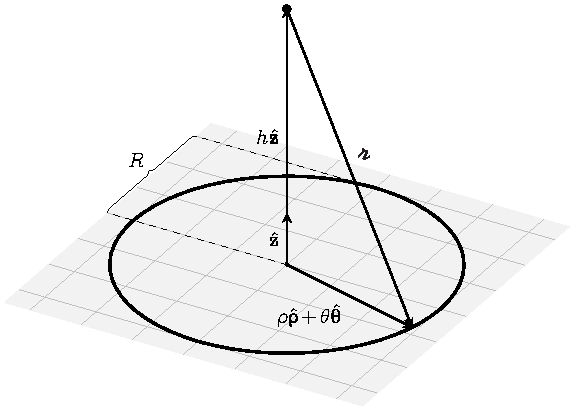
\includegraphics{perfect-dipole-over-loop.pdf}
	\caption{Perfect magnetic dipole hovering at a height $h$ over a loop radius $R$.}
	\label{fig:perfect-dipole-over-loop}
\end{figure}
Since we want to find the magnetic flux over a copper wire illustrated in \cref{fig:perfect-dipole-over-loop}, $\brc$ must be a vector that points from the magnet to any arbitrary points in the wire. Geometrically, $h\zhat + \brc = \rho\phat + \theta\that$; thus,
\begin{equation}
	\brc = \rho\phat + \theta\that - h\zhat.
\end{equation}
Using $\vv{m} = -m\zhat$,
\begin{align}
	\vv{B}(\brc) &= \frac{\bperm}{4\cpi}\ab[\frac{3\brc(-m\zhat\vdot(\rho\phat + \theta\that - h\zhat))}{\rc^5} + \frac{m\zhat}{\rc^3}] \\
				 &= \frac{\bperm}{4\cpi}\ab[\frac{3\brc}{\rc^5}(mh) + \frac{m\zhat}{\rc^3}] \\
	\vv{B}(\brc) \cdot \zhat &= \frac{\bperm}{4\cpi}\ab[\frac{3mh}{\rc^5}(\brc\vdot\zhat) + \frac{m}{\rc^3}(\zhat\vdot\zhat)] \\
							 &= \frac{\bperm}{4\cpi}\ab[\frac{1}{\rc^3} - \frac{3h^2}{\rc^5}]
\end{align}
The magnetic flux over the disk is then
\begin{align}
	\mflux &= \int\limits_{0}^{2\cpi}\int\limits_{0}^{R}\ab[\vv{B}(\brc)\cdot\zhat]\rho\odif{\rho}\odif{\theta} \\
		   &= \frac{\bperm m}{4\cpi} \int\limits_{0}^{2\cpi}\int\limits_{0}^{R}\ab(\frac{1}{\rc^3} - \frac{3h^2}{\rc^5})\rho\odif{\rho}\odif{\theta} \\
		   &= \frac{\bperm m}{4\cpi} \int_0^{2\cpi}\odif{\theta} \times \ab[
		   \int_0^{R}\frac{\rho}{(\rho^2 + h^2)^{\frac{3}{2}}}\odif{\rho} - 3h^2\int_0^R\frac{\rho}{(\rho^2 + h^2)^{\frac{5}{2}}}\odif{\rho}
		   ] \\
		   &= \frac{\bperm m}{2}\ab[\peval{-\frac{1}{(\rho^2 + h^2)^{\frac{1}{2}}}}_0^R - 3h^2\peval{ - \frac{1}{3}\times\frac{1}{(\rho^2 + h^2)^{\frac{3}{2}}}}_0^R] \\
		   &= -\frac{\bperm m}{2}\ab[-\frac{1}{(R^2 + h^2)^{\frac{1}{2}}} + \frac{1}{h} + h^2\ab(\frac{1}{(R^2 + h^2)^{\frac{3}{2}}} - \frac{1}{h^3})] \\
		   &= -\frac{\bperm m}{2}\ab[\frac{h^2}{(R^2 + h^2)^{\frac{3}{2}}} - \frac{1}{(R^2 + h^2)^{\frac{1}{2}}}]
\end{align}
The change in magnetic flux is proportional to the electromotive force, which is distributed throughout the wire. If the wire is wounded around $N$ times, the electromotive force is also multiplied by $N$. At a certain height $h$,
\begin{align}
	\emf &= -N\odv{\mflux}{t} \\
		 &= -\frac{N\bperm m}{2}\ab[\odv*{\frac{h^2}{(R^2 + h^2)^{\frac{3}{2}}}}{t} - \odv*{\frac{1}{(R^2 + h^2)^{\frac{1}{2}}}}{t}] \\
		 &= -\frac{N\bperm m}{2}\ab[\ab(\frac{2h}{(R^2 + h^2)^{\frac{3}{2}}} - \frac{3h^3}{(R^2 + h^2)^{\frac{5}{2}}})\odv{h}{t} - \frac{h}{(R^2 + h^2)^{\frac{3}{2}}}\odv{h}{t}] \\
		 &= -\frac{N\bperm mh}{2}\odv{h}{t}\ab[\frac{1}{(R^2 + h^2)^{\frac{3}{2}}} - \frac{3h^2}{(R^2 + h^2)^{\frac{5}{2}}}] \label{eq:theoretical-voltage}
\end{align}

In a wire, $\emf$ is identical to $V$, the voltage. By Ohm's law, $V = I\Omega$, the current induced by a perfect magnetic dipole falling is
\begin{align}
	I &= -\frac{N\bperm mh}{2\Omega}\odv{h}{t}\ab[\frac{1}{(R^2 + h^2)^{\frac{3}{2}}} - \frac{3h^2}{(R^2 + h^2)^{\frac{5}{2}}}].
\end{align}
The Biot-Savart law states that the magnetic field generated by a current $I$ is given by
\begin{equation}
	\vv{B}'(\brc) = \frac{\bperm}{4\cpi}\cint\frac{I\odif{\vv{l}} \times \brc'}{|\brc'|^3}\odif{\brc'}.
\end{equation}
The system that we're interested in: magnetic field directly above a ring with uniformed current distribution, has a very well-known result in electrodynamics: \lcite{griffiths-2023}
\begin{equation}
	\vv{B}(h\zhat) = \frac{\bperm I}{2}\frac{R^2}{(R^2 + z^2)^{\frac{3}{2}}}\zhat \label{eq:b-field-over-loop}
\end{equation}
We can use this result to directly evaluate the force that the ring acts on the magnetic dipole.

A magnet in an external magnetic field experiences a force that follows the direction of the external field's gradient: \lcite{boyer-1988}
\begin{equation}
	\vv{F} = \grad(\vv{m}\cdot\vv{B})
\end{equation}
where $\vv{m}$ is of the magnet that experiences the force. From \cref{eq:b-field-over-loop},
\begin{align}
	\vv{m}\cdot\vv{B} &= -m\zhat\cdot\vv{B} \\
					  &= -\frac{m\bperm I}{2}\frac{R^2}{(R^2 + z^2)^{\frac{3}{2}}},
\end{align}
and
\begin{align}
	&\grad(\vv{m}\cdot\vv{B}) \nonumber\\
	&= \ab[\xhat\pdv{}{x} + \yhat\pdv{}{y} + \zhat\pdv{}{z}]\ab(-\frac{m\bperm I}{2}\frac{R^2}{(R^2 + z^2)^{\frac{3}{2}}}) \\
	&= \zhat\pdv*{\ab(-\frac{m\bperm I}{2}\frac{R^2}{(R^2 + z^2)^{\frac{3}{2}}})}{z} \\
	&= -\frac{m\bperm}{2}\pdv*{\ab(-\frac{N\bperm mz}{2\Omega}\odv{z}{t}\ab[\frac{1}{(R^2 + z^2)^{\frac{3}{2}}} - \frac{3z^2}{(R^2 + z^2)^{\frac{5}{2}}}]\frac{R^2}{(R^2 + z^2)^{\frac{3}{2}}})}{z}\zhat \nonumber\\
	&= \ab(\frac{m\bperm}{2})^2\frac{NR^2}{\Omega}\odv{z}{t}\odv*{\ab(\frac{1}{(R^2 + z^2)^{3}} - \frac{3z^2}{(R^2 + z^2)^4})}{z} \\
	&= \frac{NR^2}{\Omega}\ab(\frac{m\bperm}{2})^2\ab(\frac{24z^3}{(R^2 + z^2)^5} + \frac{12z}{(R^2 + z^2)^4})\odv{z}{t}
\end{align}
The term $\odv{z}{t}$ must be obtained via Newton's second law. Let $M$ be the mass of the magnet, then
\begin{align}
	\vv{F} &= M\odv[ord = 2]{z}{t} \\
	M\odv[ord = 2]{z}{t} &= \ab(\frac{m\bperm}{2})^2\frac{NR^2}{\Omega}\ab(\frac{24z^3}{(R^2 + z^2)^5} + \frac{12z}{(R^2 + z^2)^4})\odv{z}{t} - Mg \\
	\odv[ord = 2]{z}{t} &= \ab(\frac{m\bperm}{2})^2\frac{12NR}{\Omega M}\ab(\frac{2z^3}{(R^2 + z^2)^5} + \frac{z}{(R^2 + z^2)^4})\odv{z}{t} - g
\end{align}
I shall let
\begin{gather}
	\alpha \equiv \ab(\frac{m\bperm}{2})^2\frac{12NR}{\Omega M}, \\
	f(z) \equiv \frac{2z^3}{(R^2 + z^2)^5} + \frac{z}{(R^2 + z^2)^4};
\end{gather}
therefore,
\begin{equation}
	\ddot{z} = \alpha f(z)\dot{z} - g
\end{equation}
By using the chain rule, the differential equation can be reduced into a first-order nonlinear ordinary differential equation.
\begin{align}
	\odv[ord = 2]{z}{t} &= \alpha f(z)\dot{z} - g \\
	\odv{\dot{z}}{z}\odv{z}{t} &= \alpha f(z)\dot{z} - g \\
	\dot{z}\odv{\dot{z}}{z} &= \alpha f(z)\dot{z} - g.
\end{align}
This is the Abel's equation of the second form, which unfortunately has no analytical solution in this case. Therefore, some terms must be neglected or approximated.

\section{Neglection of the Lenz's law}

The term $\alpha$ has a magnitude of around $10^{-20}$, which is merely impossible to detect. Therefore, one could say that if a solenoid is lengthless, it's almost impossible to detect the contribution from the Lenz's law. If that's neglected, the differential equation reads
\begin{equation}
	\ddot{z} = -g,
\end{equation}
which has a pretty well known result in classical mechanics:
\begin{gather}
	\dot{z} = v_0 - gt, \\
	z = z_0 + v_0t - \frac{1}{2}gt^2,
\end{gather}
where $v_0$ is the initial velocity and $z_0$, the initial height. Since we're dropping the magnet from zero velocity,
\begin{equation}
	\dot{z} = -gt \mathand z = z_0 - \frac{1}{2}gt^2. \label{eq:lenz-law-neglection-zzdot}
\end{equation}

As said in \cref{sec:problem-statement}, we're interested in measuring the difference between the maxima and the minima of the voltage. When the contribution from Lenz's law is neglected, we can directly substitute \cref{eq:lenz-law-neglection-zzdot} into the voltage equation \cref{eq:theoretical-voltage}, (repeated for ease of reading)
\begin{equation*}
	\emf = -\frac{N\bperm mz}{2}\odv{z}{t}\ab[\frac{1}{(R^2 + z^2)^{\frac{3}{2}}} - \frac{3z^2}{(R^2 + z^2)^{\frac{5}{2}}}]
\end{equation*}
to get\footnote{Courtesy the \texttt{SymPy} package in \texttt{Python} language for letting me evaluate these without a hassle.}
\begin{align}
	\emf &\approx \begin{multlined}[t]
		 -\frac{N\bperm m(z_0 - \frac{1}{2}gt^2)}{2}(-gt) \times \\ 
		\ab[\frac{1}{\ab(R^2 + \ab(z_0 - \frac{1}{2}gt^2)^2)^{\frac{3}{2}}} - \frac{3h^2}{\ab(R^2 + \ab(z_0 - \frac{1}{2}gt^2)^2)^{\frac{5}{2}}}]
	\end{multlined} \\
		 &= -4N\bperm gmt \frac{\ab(2R^2 - \ab(gt^2 - 2z_0)^2)\ab(gt^2 - 2z_0)}{\ab(4R^2 + \ab(gt^2 - 2z_0)^2)^{\frac{5}{2}}}
\end{align}
The next step is to take the derivative of the electromotive force w.r.t. time and find the position in which this derivative equals zero. Since we're only interested in $\odv{\emf}{t} = 0$, the actual derivative isn't required. The derivative of each function that makes up $\emf$ is already enough to do so.

Let
\begin{gather}
	f_1 \equiv t(gt^2 - 2z_0), \quad \odv{f_1}{t} = 3gt^2 - 2z_0, \\
	f_2 \equiv 2R^2 - (gt^2 - 2z_0)^2, \quad \odv{f_2}{t} = -4gt(gt^2 - 2z_0), \\
	f_3 \equiv \ab(4R^2 + \ab(gt^2 - 2z_0)^2)^{-\frac{5}{2}}, \quad \odv{f_3}{t} = -\frac{10gt(gt^2 - 2z_0)}{\ab(4R^2 + (gt^2 - 2z_0)^2)^{\frac{7}{2}}} .
\end{gather}
The product rule for three functions says
\begin{equation}
	\odv*{(f_1f_2f_3)}{t} = f_1f_2f_3\ab(\frac{1}{f_1}\odv{f_1}{t} + \frac{1}{f_2}\odv{f_2}{t} + \frac{1}{f_3}\odv{f_3}{t})
\end{equation}
For this derivative to be zero, either $f_1$, $f_2$, $f_3$, or $\textstyle\ab(\frac{1}{f_1}\odv{f_1}{t} + \frac{1}{f_2}\odv{f_2}{t} + \frac{1}{f_3}\odv{f_3}{t})$ must be zero. However, when $f_1$, $f_2$ and $f_3$, are zero, it also represents the root of $\emf$, which doesn't have zero derivative. Therefore, we're only interested in the case where $\textstyle\ab(\frac{1}{f_1}\odv{f_1}{t} + \frac{1}{f_2}\odv{f_2}{t} + \frac{1}{f_3}\odv{f_3}{t})$ is zero.

Funnily enough, the equation
\begin{equation}
	\begin{multlined}
		0 = f_1f_2f_3\ab(\frac{1}{f_1}\odv{f_1}{t} + \frac{1}{f_2}\odv{f_2}{t} + \frac{1}{f_3}\odv{f_3}{t}) = \\
		-\frac{10gt(gt^2 - 2z_0)}{4R^2 + (gt^2 - 2z_0)^2} - \frac{4gt(gt^2 - 2z_0)}{2R^2 - (gt^2 - 2z_0)^2} + \frac{3gt^2 - 2z_0}{t(gt^2 - 2z_0)}
	\end{multlined}
\end{equation}
also doesn't have any analytical solution for $t$. Therefore, we resort to numerical methods, shown in \cref{sec:data-analysis}

